%%%%%%%%%%%%%%%%%%%%%%%%%%%%%%%%%%%%%%%%%
% University Assignment Title Page 
% LaTeX Template
% Version 1.0 (27/12/12)
%
% This template has been downloaded from:
% http://www.LaTeXTemplates.com
%
% Original author:
% WikiBooks (http://en.wikibooks.org/wiki/LaTeX/Title_Creation)
%
% License:
% CC BY-NC-SA 3.0 (http://creativecommons.org/licenses/by-nc-sa/3.0/)
% 
% Instructions for using this template:
% This title page is capable of being compiled as is. This is not useful for 
% including it in another document. To do this, you have two options: 
%
% 1) Copy/paste everything between \begin{document} and \end{document} 
% starting at \begin{titlepage} and paste this into another LaTeX file where you 
% want your title page.
% OR
% 2) Remove everything outside the \begin{titlepage} and \end{titlepage} and 
% move this file to the same directory as the LaTeX file you wish to add it to. 
% Then add \input{./title_page_1.tex} to your LaTeX file where you want your
% title page.
%
%%%%%%%%%%%%%%%%%%%%%%%%%%%%%%%%%%%%%%%%%
%\title{Title page with logo}
%----------------------------------------------------------------------------------------
%	PACKAGES AND OTHER DOCUMENT CONFIGURATIONS
%----------------------------------------------------------------------------------------

\documentclass[12pt]{article}
\usepackage[english]{babel}
\usepackage[utf8x]{inputenc}
\usepackage{amsmath}
\usepackage{graphicx}
\usepackage[colorinlistoftodos]{todonotes}
\usepackage{geometry}
\geometry{left=2cm, right=2cm, top=2cm, bottom=2cm}
\usepackage[colorlinks,linkcolor=blue,anchorcolor=blue,citecolor=blue]{hyperref}
\usepackage{float}
\usepackage{subfigure}
\setlength{\parindent}{0pt}
\setlength{\parskip}{1em}
\usepackage{enumitem}
\setitemize[1]{itemsep=0pt,partopsep=0pt,parsep=1pt,topsep=1pt}

\begin{document}

\begin{titlepage}

\newcommand{\HRule}{\rule{\linewidth}{0.5mm}} % Defines a new command for the horizontal lines, change thickness here

\center % Center everything on the page
 
%----------------------------------------------------------------------------------------
%	HEADING SECTIONS
%----------------------------------------------------------------------------------------

\textsc{\LARGE Brown University}\\[1.5cm] % Name of your university/college
\textsc{\Large cs1951-A Final Report}\\[0.5cm] % Major heading such as course name


%----------------------------------------------------------------------------------------
%	TITLE SECTION
%----------------------------------------------------------------------------------------

\HRule \\[0.4cm]
{ \large \bfseries UFO Sighting Analysis based on Weather and Geo Information}\\[0.4cm] % Title of your document
\HRule \\[1.5cm]
 
%----------------------------------------------------------------------------------------
%	AUTHOR SECTION
%----------------------------------------------------------------------------------------

\begin{minipage}{0.4\textwidth}
\begin{flushleft} \large
\emph{Author:}\\
Jin \textsc{Yan}\\
Lei \textsc{Tian}\\
Yao \textsc{Yao}\\
Jing \textsc{Qian}\\
\end{flushleft}
\end{minipage}
~
\begin{minipage}{0.4\textwidth}
\begin{flushright} \large
\emph{Supervisor:} \\
Dan \textsc{Potter}\\
Carsten \textsc{Binnig}\\
Eli \textsc{Upfal}
\end{flushright}
\end{minipage}\\[2cm]

% If you don't want a supervisor, uncomment the two lines below and remove the section above
%\Large \emph{Author:}\\
%John \textsc{Smith}\\[3cm] % Your name

%----------------------------------------------------------------------------------------
%	DATE SECTION
%----------------------------------------------------------------------------------------

{\large \today}\\[2cm] % Date, change the \today to a set date if you want to be precise

%----------------------------------------------------------------------------------------
%	LOGO SECTION
%----------------------------------------------------------------------------------------


\includegraphics[width=3cm]{figure/logo.png}\\[1cm] % Include a department/university logo - this will require the graphicx package
 
%----------------------------------------------------------------------------------------

\vfill % Fill the rest of the page with whitespace

\end{titlepage}
\section{Introduction}

These days, people are crazy about exploring habitable planets and extraterrestrial intelligence. Meanwhile, UFO events have been happening around us for decades, and people tell their UFO encounters in thousands of ways. Predicting any aspects about UFO is intriguing since these tiny fickle light dots leave us little trace behind.

In this project, we try to investigate this topic in three steps. First, we figure out correlations between UFO sightings and data from other sources, such as geometry, weather, population and territory area. Second, based on statistic analysis and machine learning techniques, we develop models to detect fake UFO reports. Finally, we build up a web application to visualize our analysis results and to provide users a way to interact with our project, such as enabling them to report their own sightings and get access to fake detection result.

The whole data pipeline of our project is illustrated in figure \ref{architecture}. For the rest part of our project report,  we will first discuss about data processing in section \ref{data}, and statistic analysis on UFO data in section \ref{statistic}. Machine learning methods will be indicated in section \ref{ml}. As for web application,  we will demonstrate the data pipeline and how our system works in section \ref{methodology}. In section \ref{challenge}, we will discuss the challenges we met during working on this project. Finally, in section \ref{conclusion}, we will claim the conclusions as well as future work. In section \ref{ack}, we give our profound acknowledgement to all people who help us with the project.

\begin{figure}[H]
    \centering
    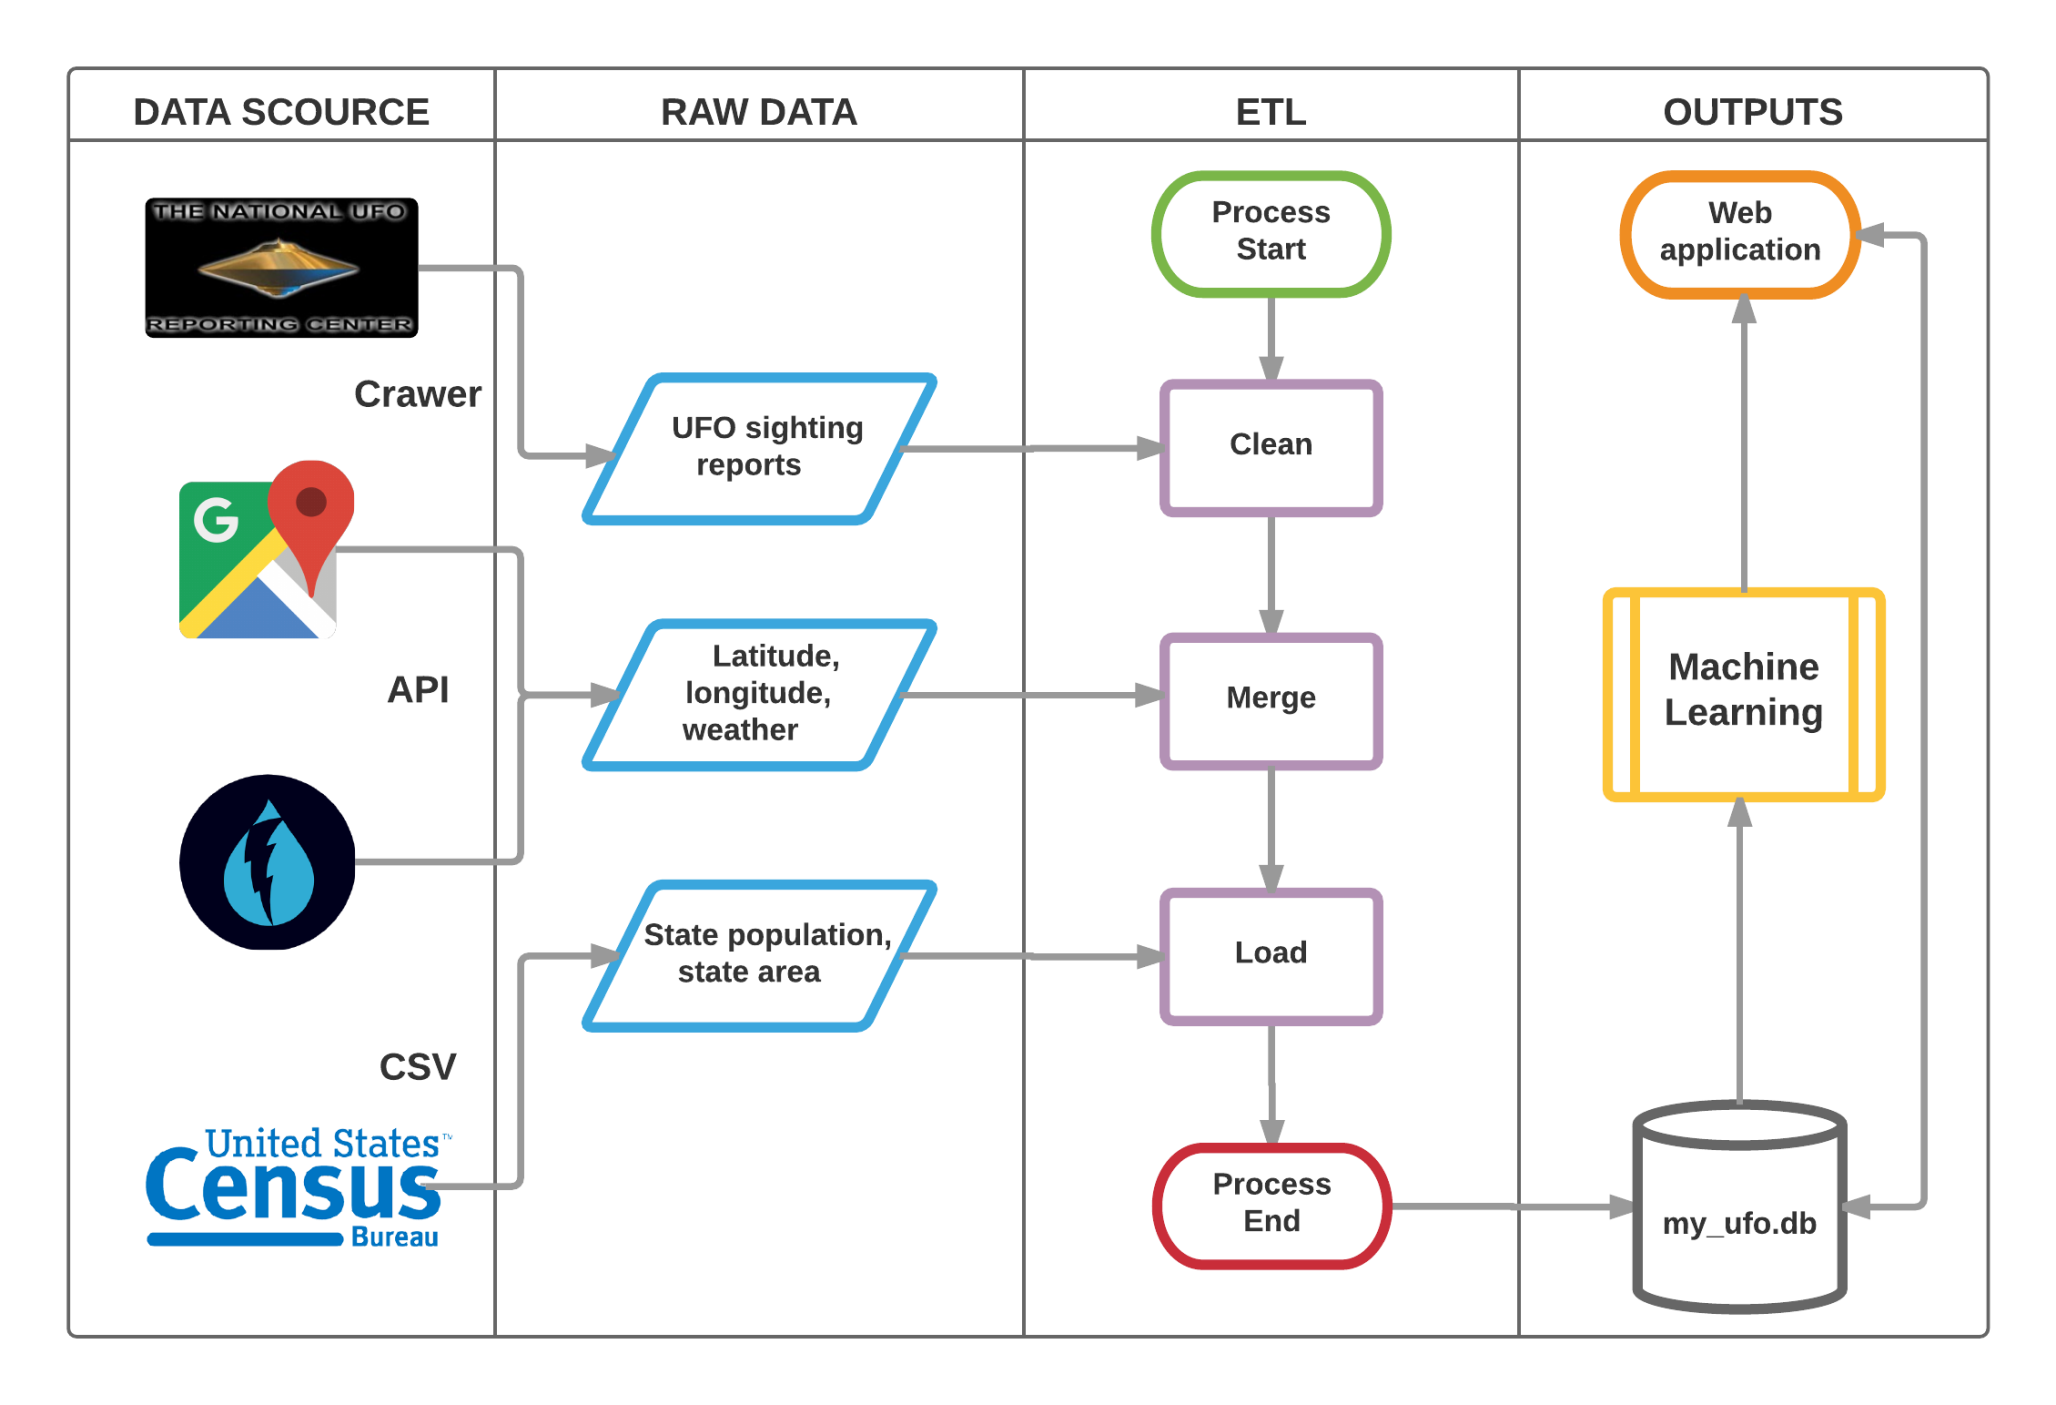
\includegraphics[width=14cm]{figure/architecture.png}
    \caption{data pipeline architecture}
    \label{architecture}
\end{figure}
\section{Data}\label{data}
\subsection{Data Source \& Collection}
Our data is collected from four different sources:

\emph{UFO Sighting Data}, the majority of our data set, is from National UFO Report Center~\cite{nuforc}. It is composed by 96000 UFO sighting reports and each report contains information of event date (year, month, day, hour), city, state, shape, duration, sighting description and posted date. Since this website doesn't provide an API to access the data, we implement a web crawler to collect data from its web pages. 

\emph{Geo Information Data} is collected from Google Map~\cite{googlemap} which provides well-developed APIs for developers to obtain comprehensive information. We first filter out cities where UFO events happened, and then obtain longitude and latitude information of these cities. In total, about 19000 records of geo information have been collected. 

\emph{Weather Data} is collected from DarkSky website~\cite{darksky}. We collect weather conditions (icon, temperature, apparent temperature, dew point, humidity, wind speed, wind bearing, visibility and pressure) when UFO events happened. Weather data has the same size with UFO sighting data.

\emph{U.S. Area/population Data} is from U.S. Census Bureau~\cite{census}. The data is downloaded manually and is stored in separate CSV files sorted by year.

\subsection{Data ETL}
A snapshot of raw UFO report data is as following:

\begin{figure}[H]
    \centering
    
\includegraphics[width=14cm]{figure/raw_event.jpg}
    \caption{raw UFO sighting data}
    \label{raw_event}
\end{figure}

We separate each fields, unify units of measurement (i.e. use seconds to measure any event duration), clean the summary, and remove records that contain invalid data elements. Also, in order to make further data processing easier, we complete the following steps for each summary field:

\begin{itemize}
    \item lowercase all characters
    \item strip punctuation
    \item remove all items in brackets
    \item apply Porter Stemming algorithm
\end{itemize}

And what's worth noting is that we use NUFORC's comments on each record's summary field to label report as true (1) or fake (0). 

In order to distinguish each data record in database, we assign an event\_id to each report data along with the weather data correlated to the sighting report. Each city is also assigned a location\_id. However, considering the growing data size and the way we use location information, city's latitude and longitude data are finally integrated into each report as two additional columns. Also, due to the size of reports and weather data, we store them in different data tables, although they share the same index event\_id. As for population and area data, since they are independent from UFO sightings, we create two other tables that do not have ids as indexes. Figure \ref{schema} shows the data schema of our database. 

\begin{figure}[H]
    \centering
    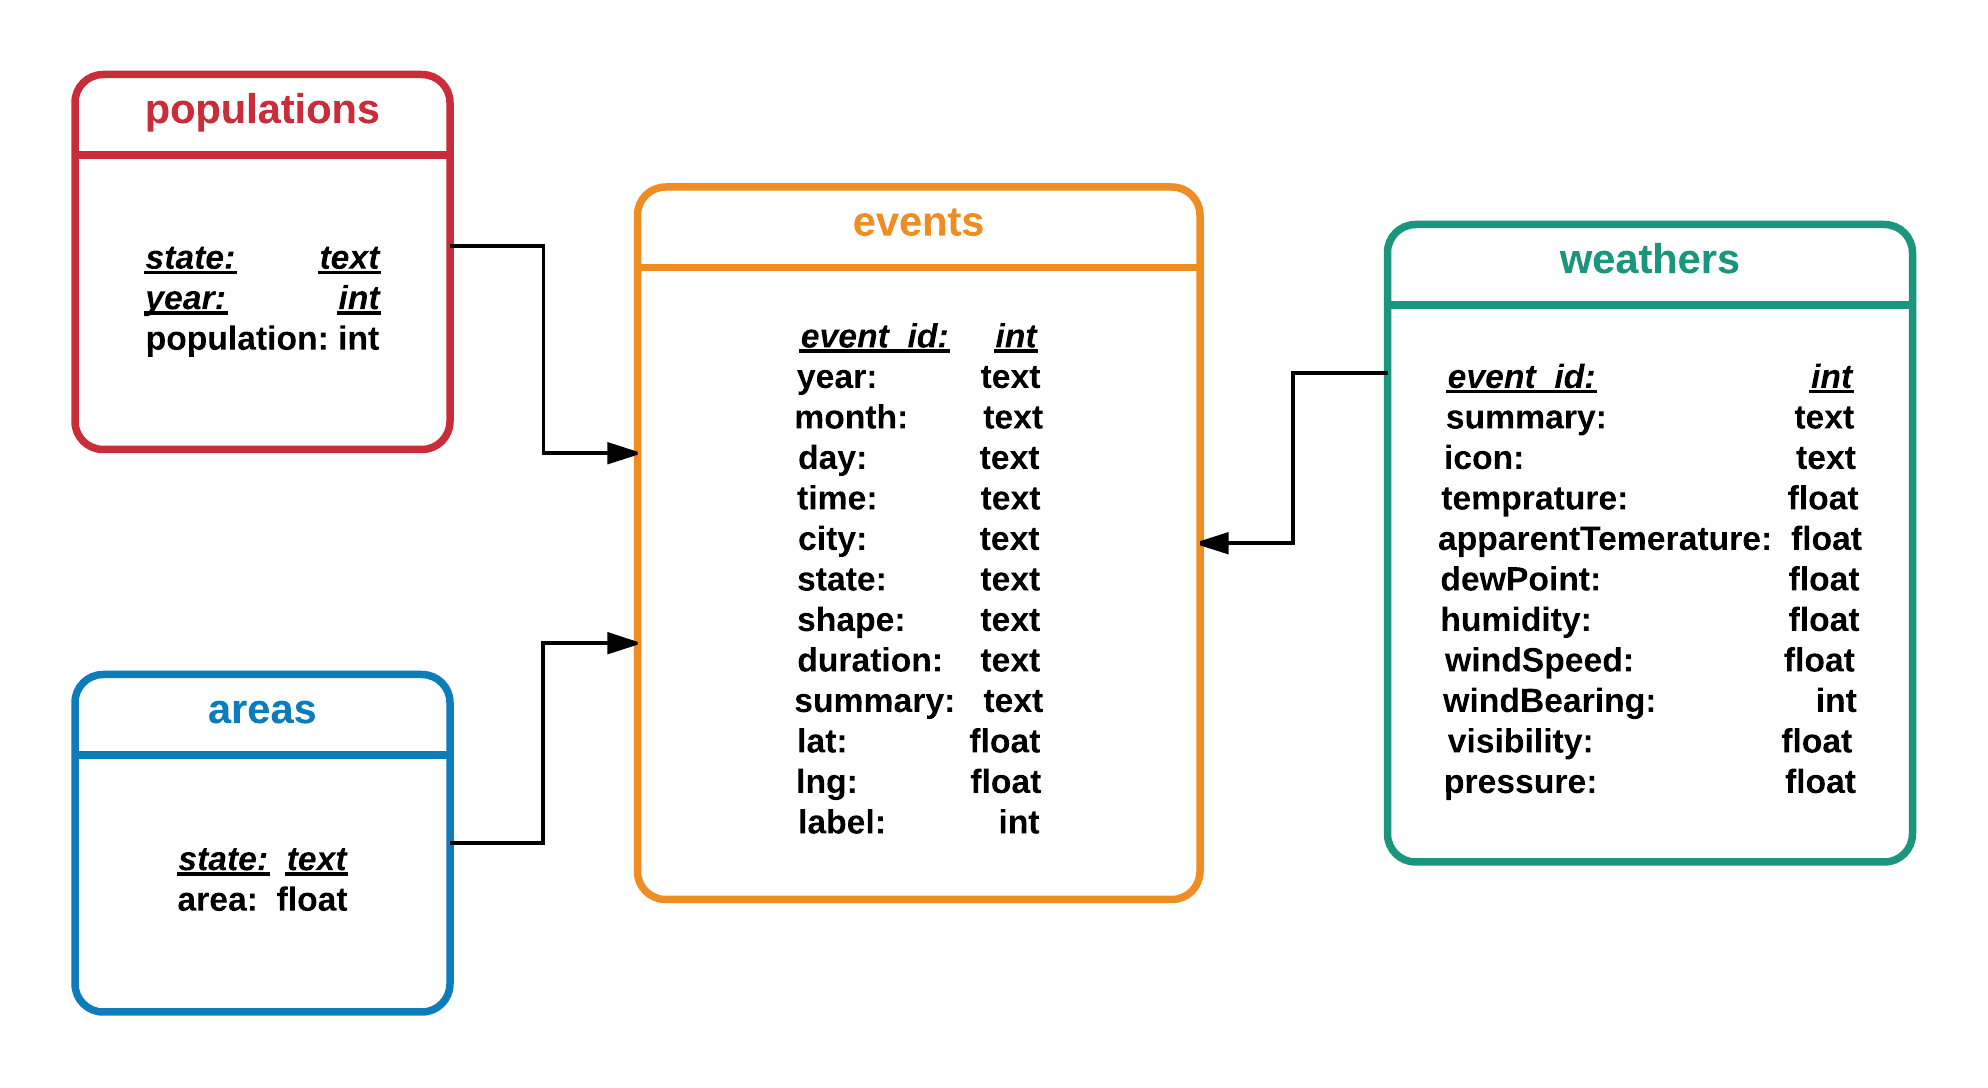
\includegraphics[width=14cm]{figure/schema.png}
    \caption{data schema of my\_ufo.db}
    \label{schema}
\end{figure}









\section{Statistic Analysis}\label{statistic}
In this section, we will discuss some statistic analysis results of UFO dataset. Figure \ref{map} and \ref{heat} demonstrate the cumulative sighting numbers from 1950 to 2016 across U.S. The UFO sightings distributed across U.S. unevenly --- California reports more UFO sightings than the other states. We believe this is because of its unique geographical conditions --- on the coast and with desert. Having the same geographical conditions, Texas, Florida and Washington also report more sightings than other states. Another kind of geographical condition, near the Great Lakes, also results in more sighting numbers, for example in Illinois, Michigan, Ohio, Pennsylvania and New York. As shown in figure \ref{mean}, we calculate estimated marginal means of duration of UFO sightings for each state. Just like what we expected, California also has an extremely high mean value than other states. 

\begin{figure}[H]
\centering 
\subfigure[state distribution]{\label{map}
\begin{minipage}[b]{0.5\textwidth}
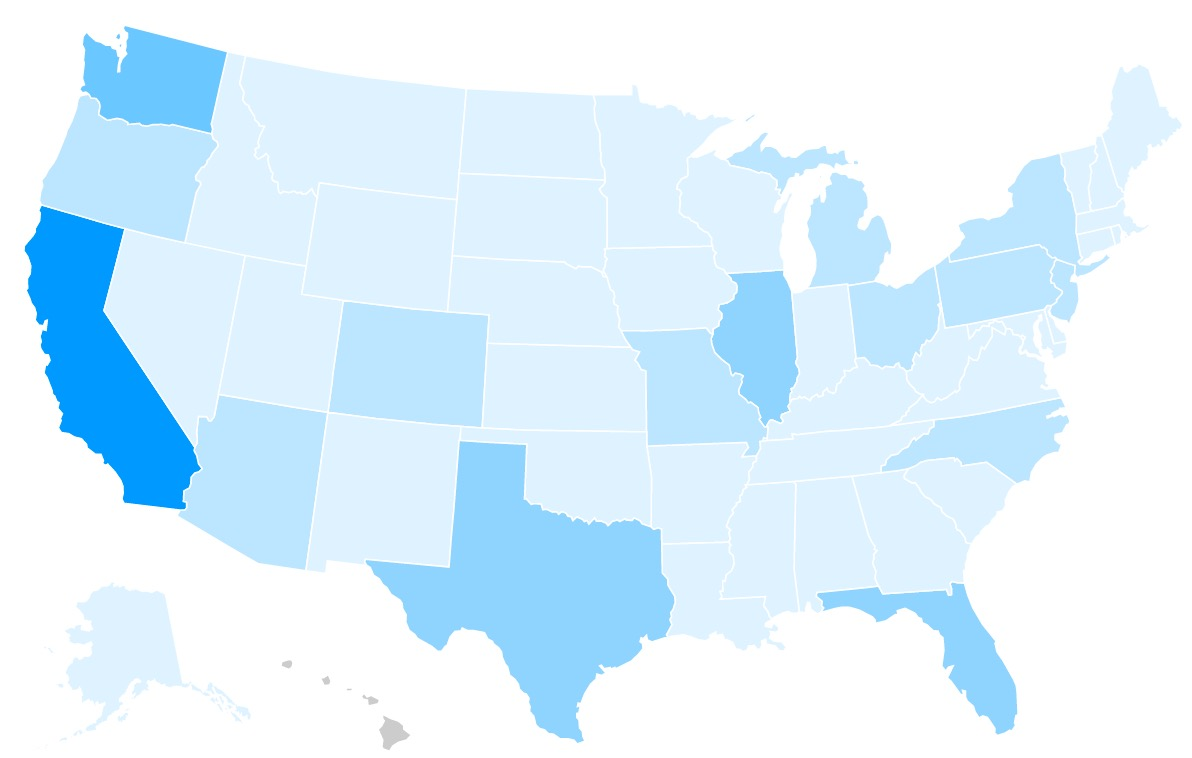
\includegraphics[width=1\textwidth]{figure/sighting_number.jpg}
\end{minipage}
}
\subfigure[heat map]{\label{heat}
\begin{minipage}[b]{0.43\textwidth}
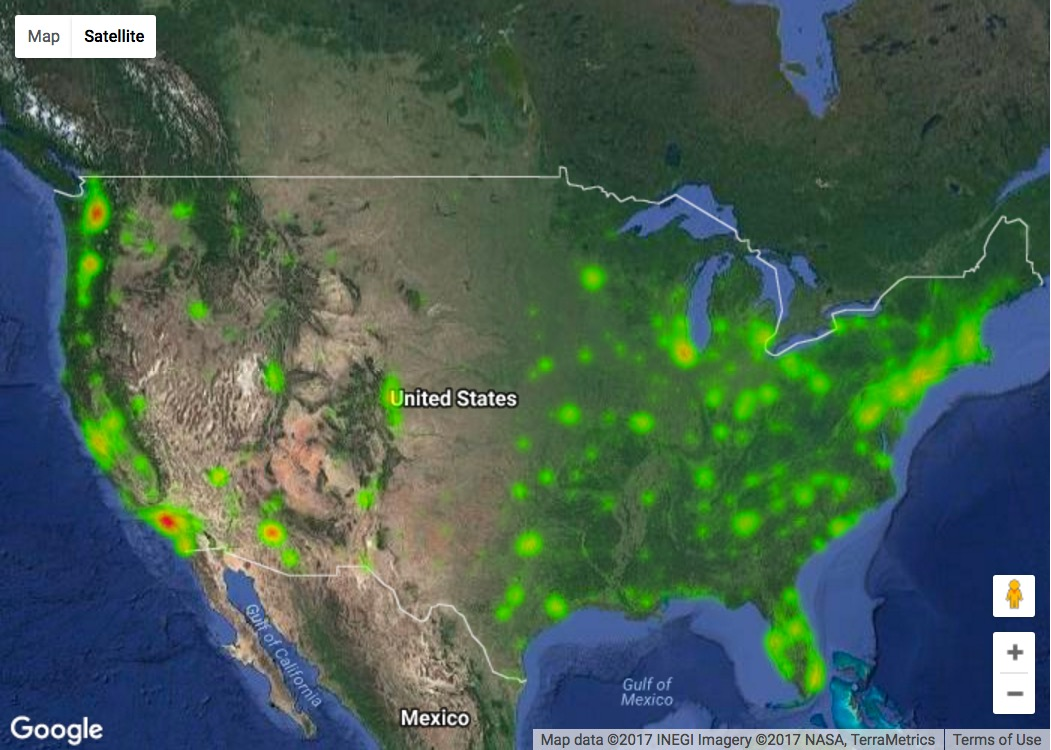
\includegraphics[width=1\textwidth]{figure/heat_map.jpg}
\end{minipage}
}
\caption{cumulative distribution around U.S.}
\end{figure}


\begin{figure}[H]
    \centering
    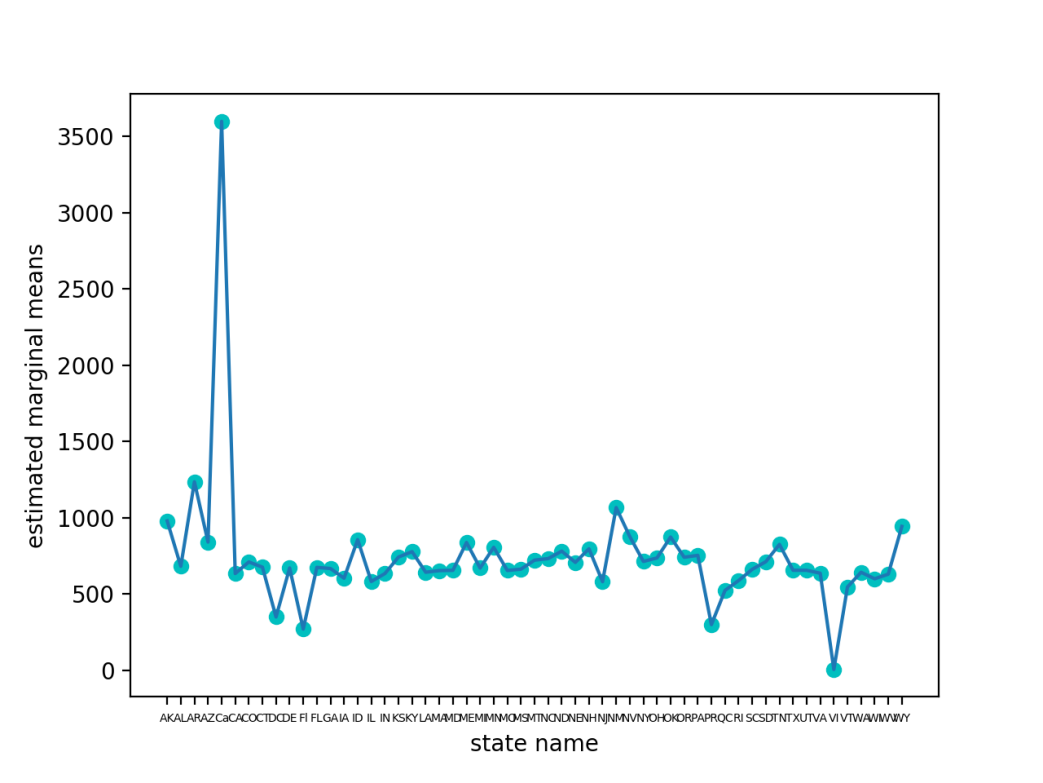
\includegraphics[width=10cm]{figure/marginal.png}
    \caption{estimated marginal means of duration for each state}
    \label{mean}
\end{figure}

Next, we analyze relations among different fields of UFO sighting reports themselves. Pie chart \ref{shape} shows that many UFO looks like light (21\%), circle (10\%) and triangle (10\%), with about 10\% witnesses are not sure about shapes. 

\begin{figure}[H]
    \centering
    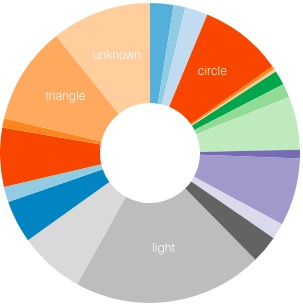
\includegraphics[width=6.5cm]{figure/shape.jpg}
    \caption{shape distribution}
    \label{shape}
\end{figure}

\begin{figure}[H]
\centering 
\subfigure[weather]{\label{weather}
\begin{minipage}[b]{0.3\textwidth}
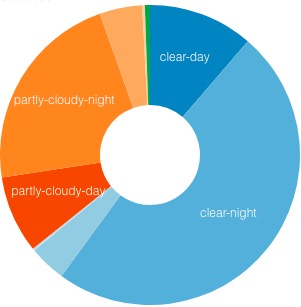
\includegraphics[width=1\textwidth]{figure/weather.jpg}
\end{minipage}
}
\subfigure[hour]{\label{hour}
\begin{minipage}[b]{0.55\textwidth}
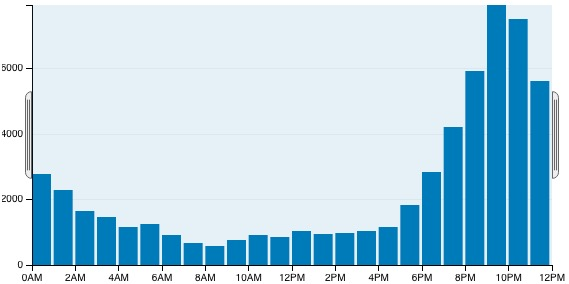
\includegraphics[width=1\textwidth]{figure/hour.jpg}
\end{minipage}
}
\subfigure[weekday]{\label{weekday}
\begin{minipage}[b]{0.55\textwidth}
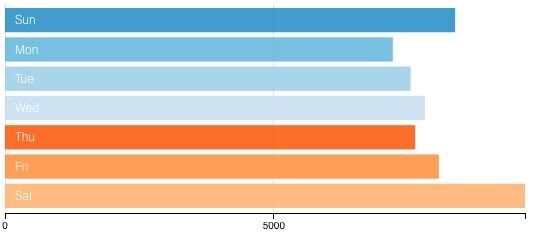
\includegraphics[width=1\textwidth]{figure/weekday.jpg}
\end{minipage}
}
\caption{weather and time distribution}
\end{figure}

For one thing, most UFO sightings occurred at night, regardless of how the weather is (as shown in figure \ref{weather}), which is consistent with figure \ref{hour} where most sightings occurred between 8 PM and 12 PM during a day. This observation reflects a basic rule about when  UFO appears --- mostly at night. For another thing, the numbers of sightings on weekends are slightly larger than those on weekdays. However, we do not accept this observation as a rule for UFO sightings. Such phenomenon happens probably because most people are busy at work on work days and they go back home early at night for rest, while they attend outdoor activities during weekend nights. Given that UFO tends to appear during the night, people have less chance to sight one during weekdays.





\section{Machine Learning}\label{ml}
\subsection{Sighting Number Regression}
In order to predict how many sightings may occur in the future, we try to find the relations between the number of sightings and other macro factors, such as area, year and population data. Figure \ref{year} shows detailed distribution of numbers of sightings from 1986 to 2016, while figure \ref{regression} shows how the number of sightings and $ln(population)$ varies relatively. It is clear that the overall number of sightings has been increasing during the last 60 years, although slightly decreased recently. However, we find there is little correlation between states' area and the numbers of their sighting reports after analyzing them thoroughly.
\begin{figure}[H]
    \centering
    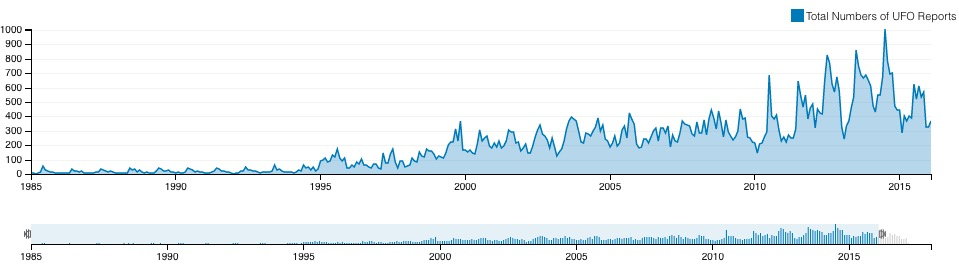
\includegraphics[width=17cm]{figure/year.jpg}
    \caption{sighting number}
    \label{year}
\end{figure}

\begin{figure}[H]
    \centering
    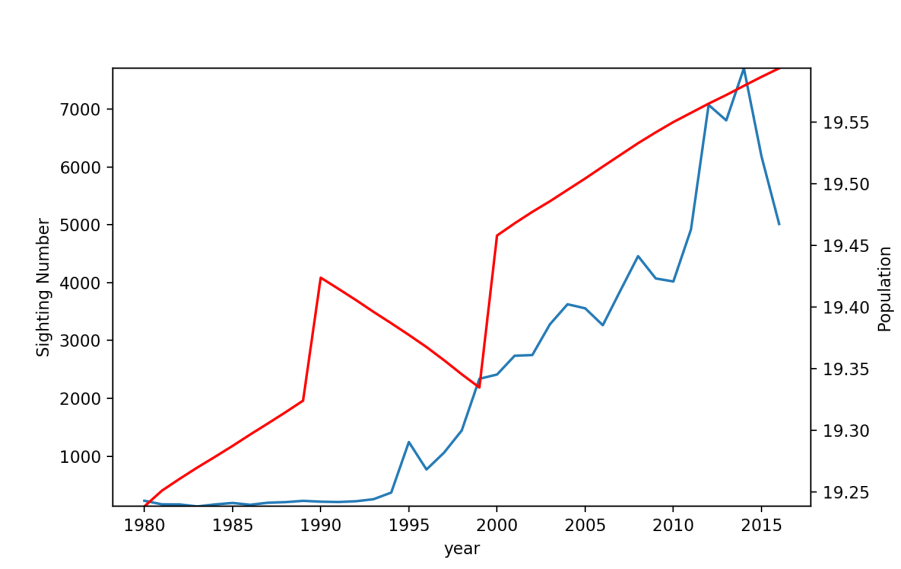
\includegraphics[width=10cm]{figure/regression.png}
    \caption{population and sighting number}
    \label{regression}
\end{figure}

We use four degree polynomial regression to fit year, total population of U.S. and total number of sightings. Generally, the result is perfect as our regression score is 0.96 out of 1. Given that the population of U.S. is 326474013 this year, we predict that there will be about 5589 UFO sightings across U.S. in 2017.

\subsection{Fake Detection}

We have encountered two main problems when working on fake detection. First, for each observation, there are two types of features --- text and numeric features, which is difficult to analyze at the same time or within the same classifier. Second, as described in section \ref{data}, each report is labeled by NUFORC's comment. However, since only a small proportion (about 5000) are labeled as fake, our data is extremely imbalanced.

To tackle the first problem, we use different classifiers for different features, and then combine all results together. After testing, we choose Decision Tree and SVM with RBF kernel to train numeric features, while using Logistic Regression and Decision Tree to train summary features. Other features, such as weather condition and shape of UFO, are quantified to numbers in order to train classifiers. For summary data, we use Porter Stemming algorithm to reduce data dimension, and then vectorize all words.

To solve the second problem, we design experiments to find out the best class weight for different classifiers. Changing class weight during training is equivalent to changing loss function: if a fake report is classified as true, a much bigger penalty will be added to the objective function. For the same reason, we also create a novel judge score, rather than only the cross validation score, to choose the best class weight, which is
$$
judge\_score = 0.7 * cross\_valid\_score + 0.3 * recall
$$
Figure \ref{classifier} shows the classifiers we use in our project. Note that except that Decision Tree model is based on text feature, the best class weight for all the other three models are around 10. This might because the number of true samples is about one order of magnitude higher than that of fake samples. Also, we find that the best judge score is from Decision Tree model regardless of the types of features we feed into classifiers. 

\begin{figure}[H]
    \centering
    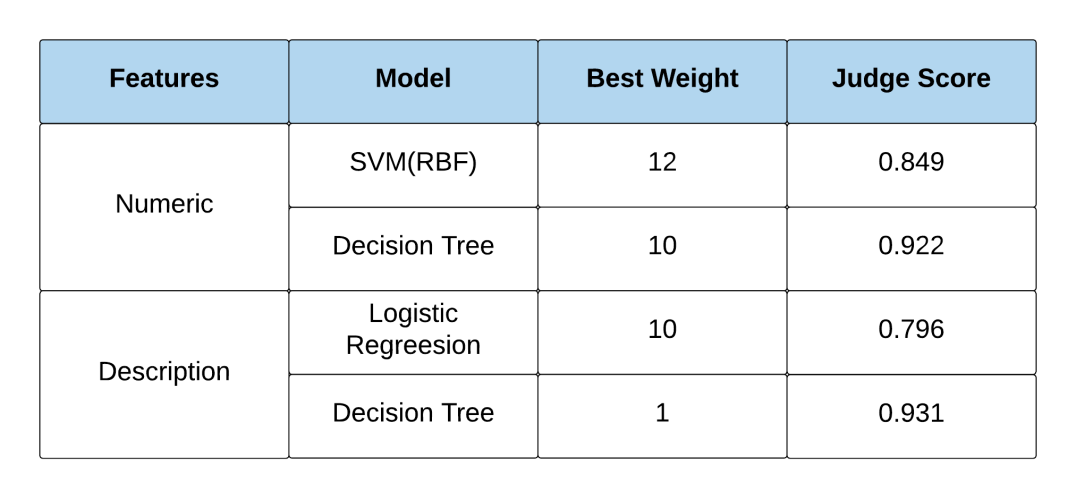
\includegraphics[width=12cm]{figure/classifier_score.png}
    \caption{classifier performance}
    \label{classifier}
\end{figure}


Figure \ref{word_weight} illustrates the words with top weights in SVM-RBF model. Here it only shows stems of words, since we apply Porter Stemming algorithm before load data into database. We can conclude that "Reptile" has the biggest positive score, while "meteor" has the biggest negative score. What surprises us is that "Miami", a state name, is regarded as one of the top positive words. Thus, we are able to make up an UFO event description that is true with high possibility: "a reptile-like alien gets off a cigarette-like spaceship in forest, and all of these are near me." While a fake description probably is: "a meteor-like ship with an alien that is unhuman."
\begin{figure}[H]
    \centering
    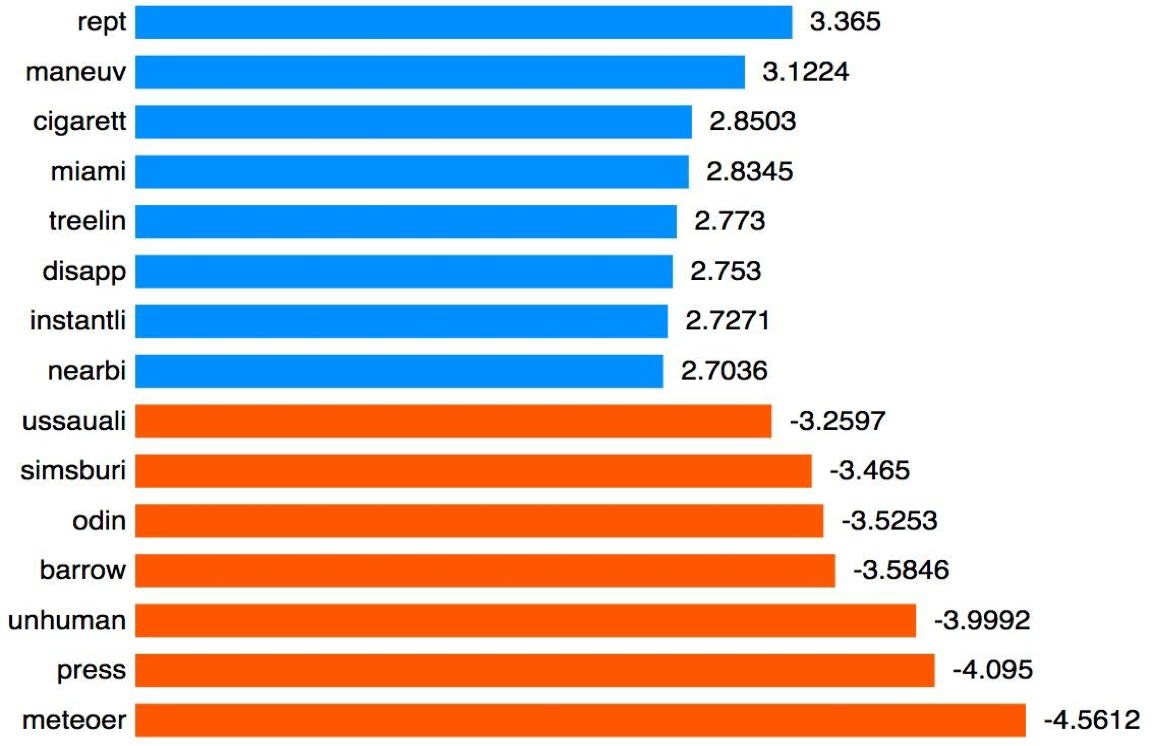
\includegraphics[width=10cm]{figure/word_weight.png}
    \caption{word weight of SVM-RBF}
    \label{word_weight}
\end{figure}


\section{Web Application}\label{methodology}

We also build a web application to interact with users. Our web application structure is shown in figure \ref{structure}. We use Node JS as web framework. For each new UFO sighting report data, we will call detection program to check it, produce truth possibility. Based on grading, we will assign true (1) or fake (0) to the report, and update my\_ufo.db. The system will periodically redo model training process based on all report data.

\begin{figure}[H]
    \centering
    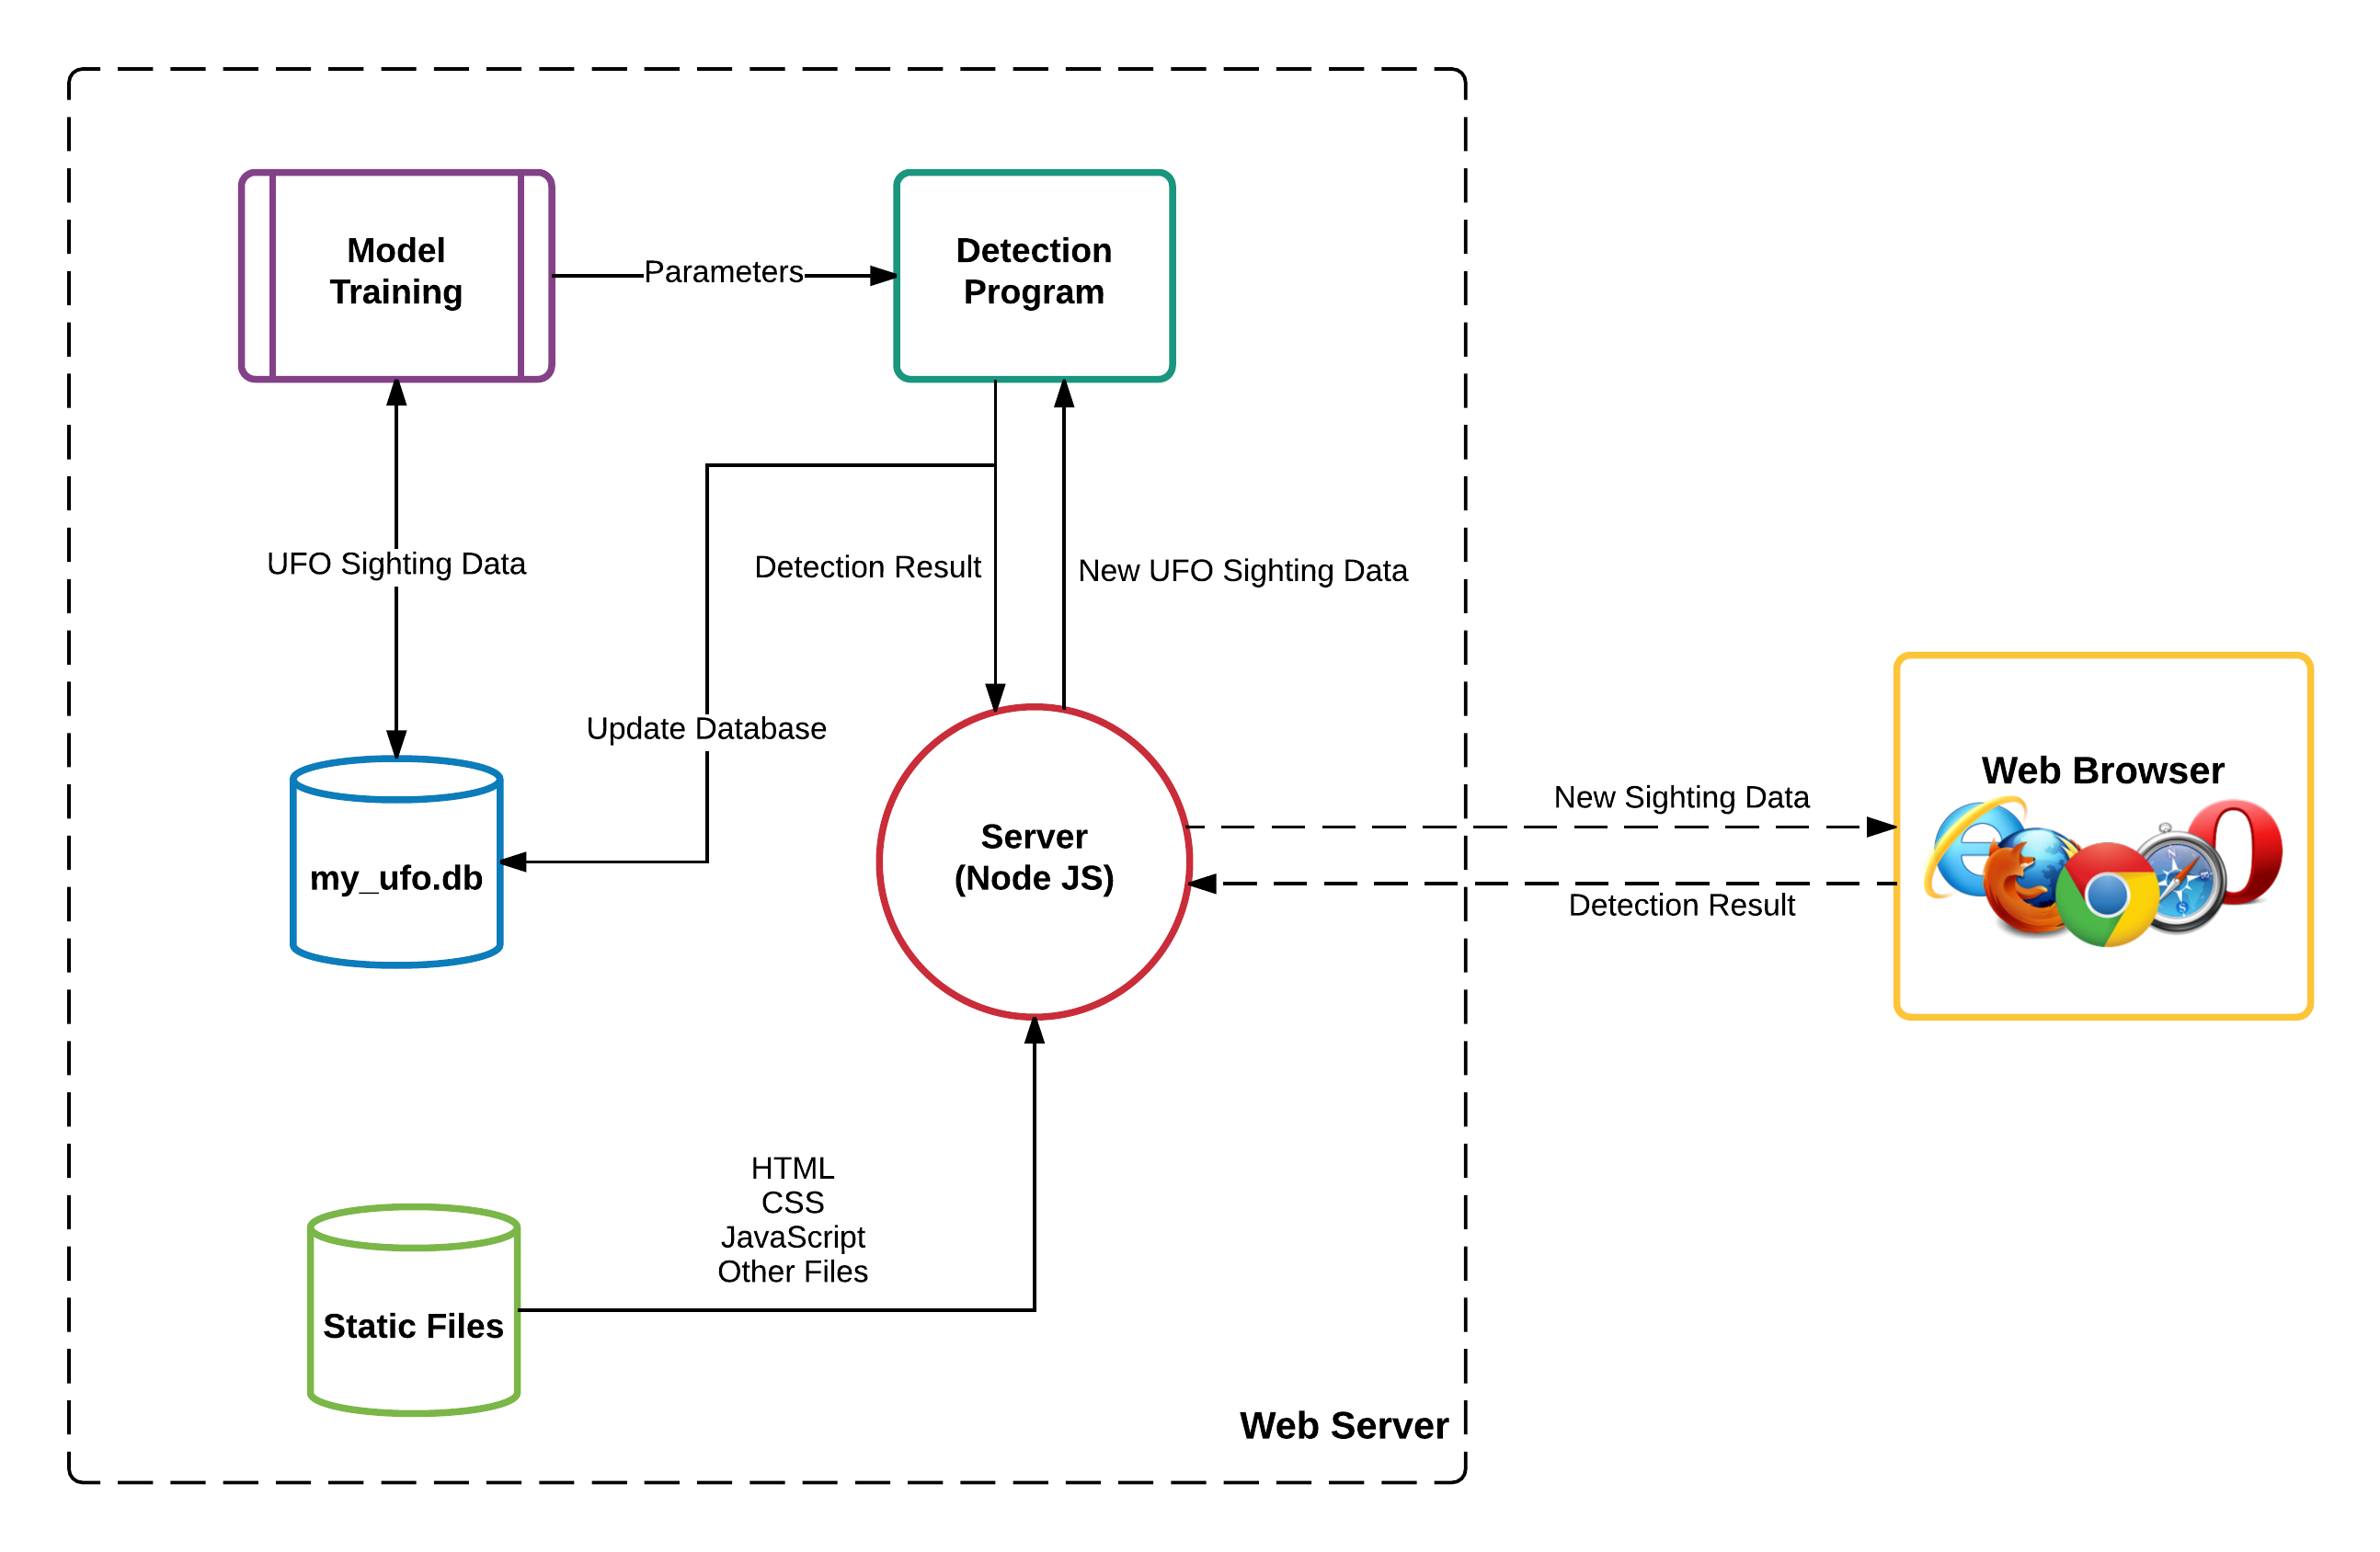
\includegraphics[width=12cm]{figure/structure.png}
    \caption{web structure}
    \label{structure}
\end{figure}

\begin{figure}
\centering 
\subfigure[home page]{\label{home}
\begin{minipage}[b]{0.6\textwidth}
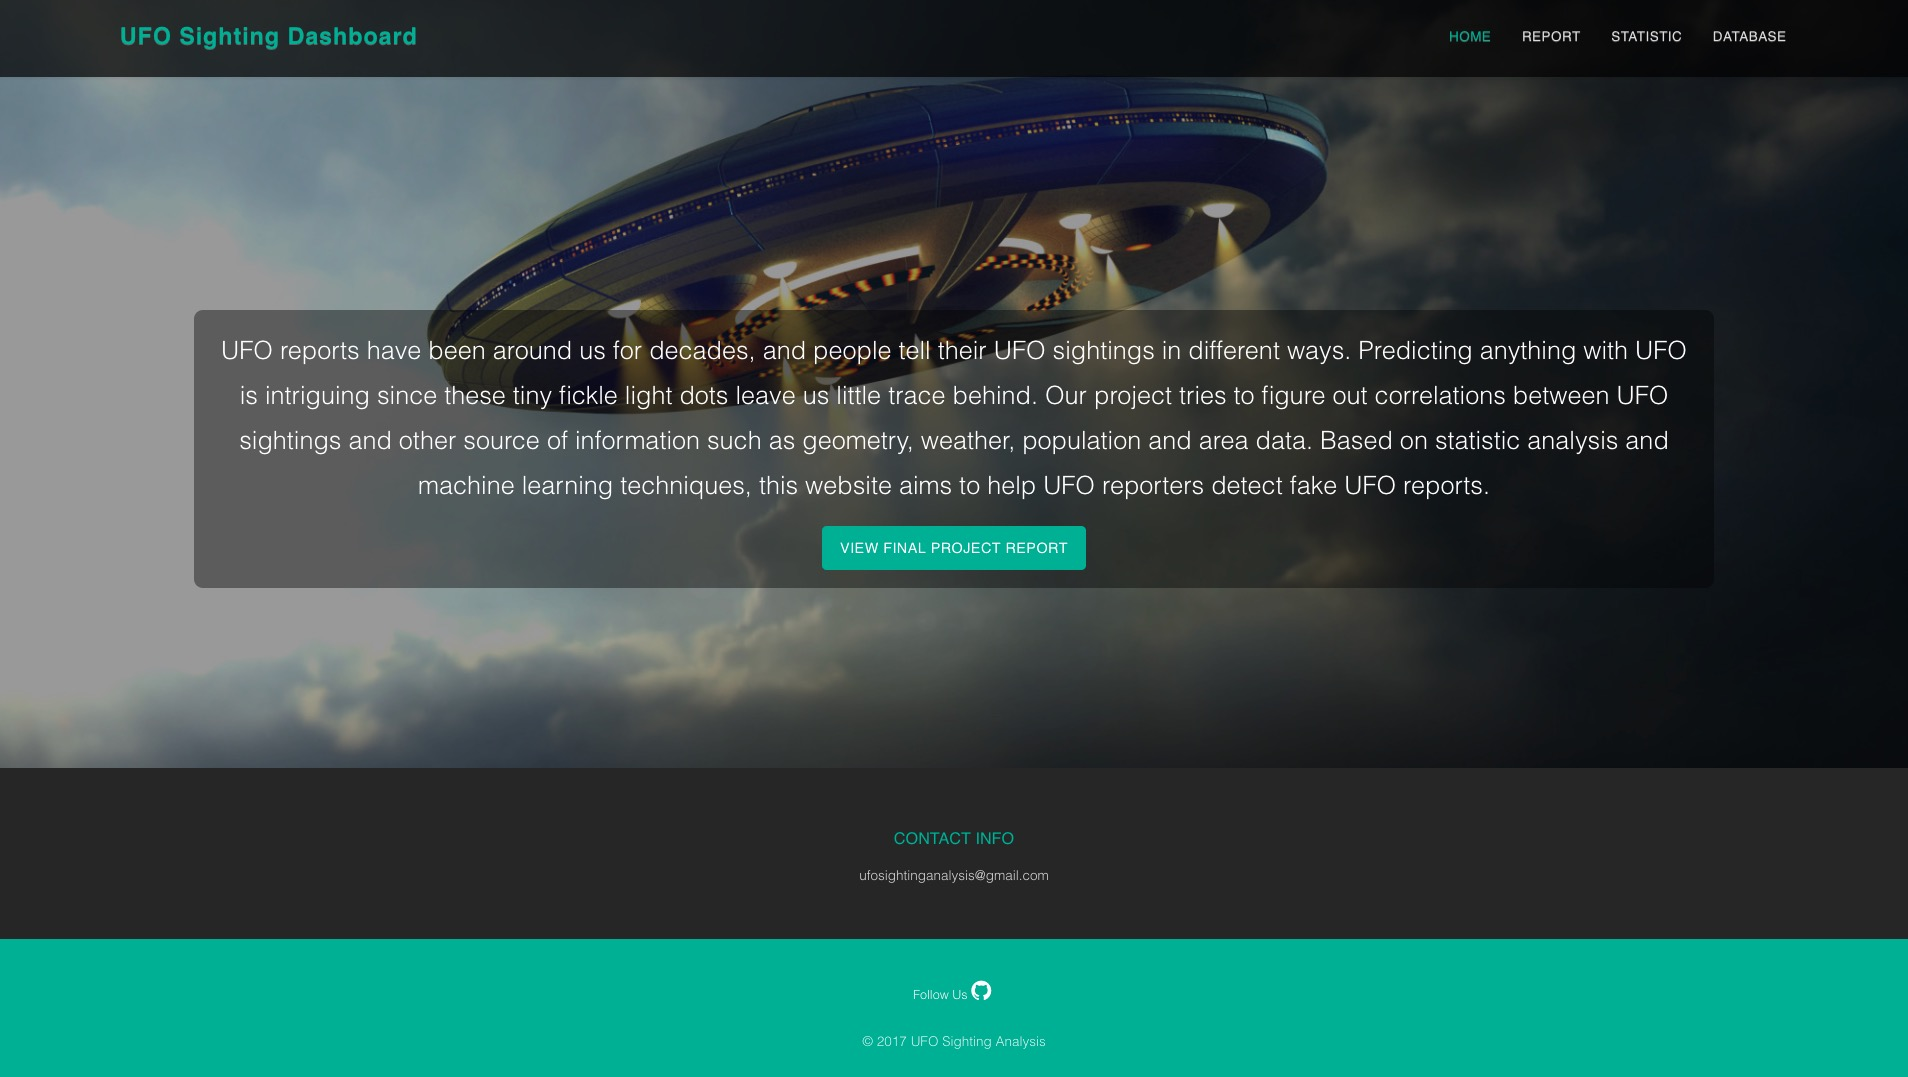
\includegraphics[width=1\textwidth]{figure/home.jpg}
\end{minipage}
}
\subfigure[statistic page]{\label{stats}
\begin{minipage}[b]{0.6\textwidth}
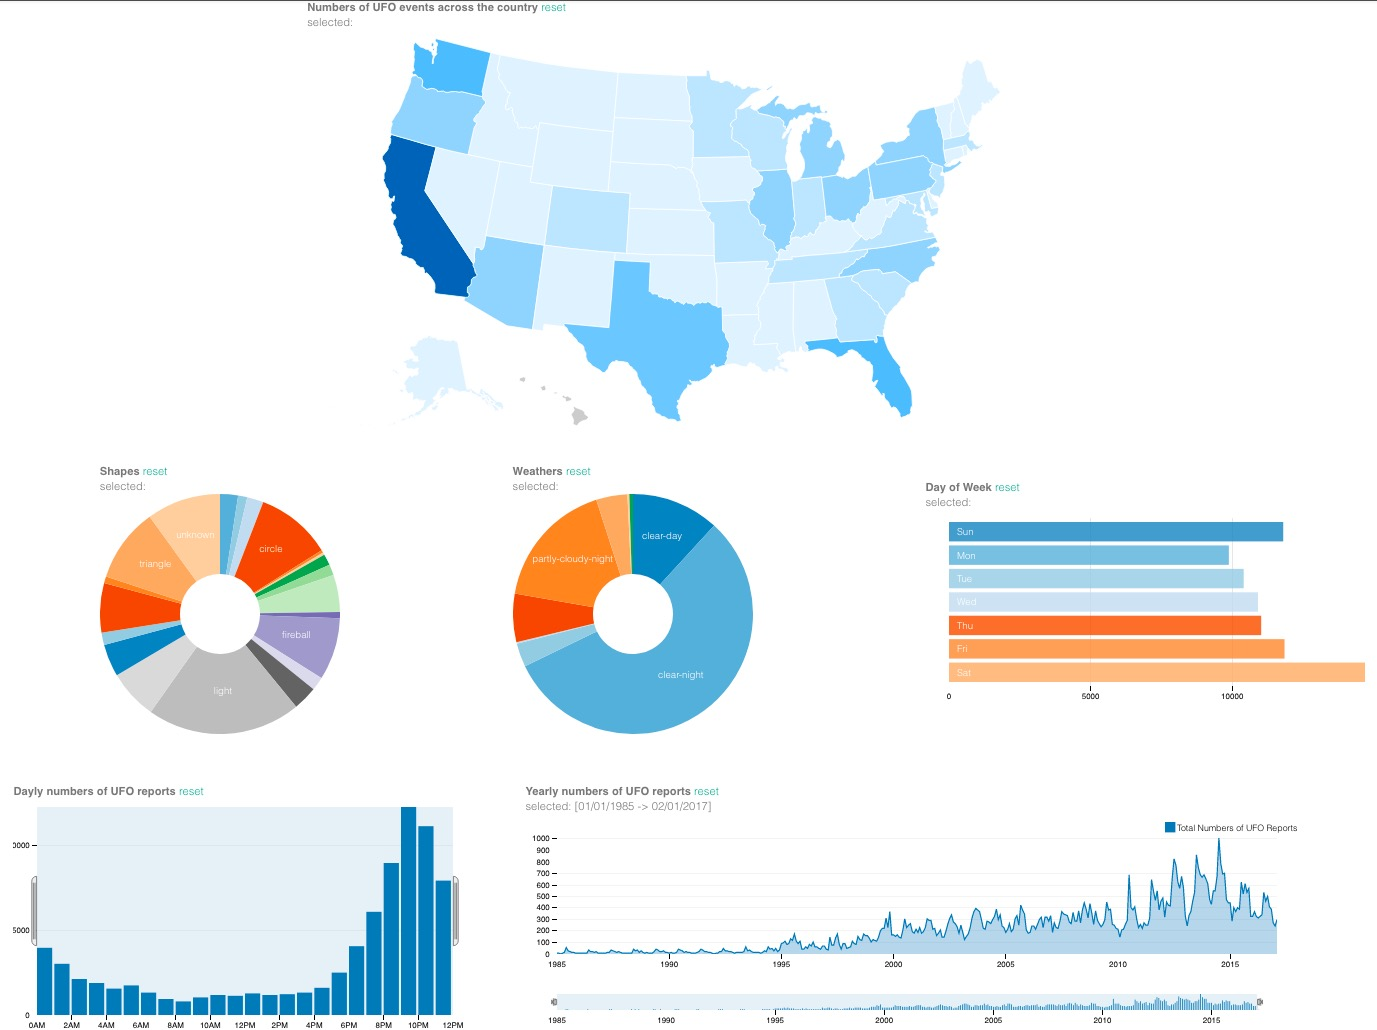
\includegraphics[width=1\textwidth]{figure/statistic.jpg}
\end{minipage}
}
\subfigure[database page]{\label{database}
\begin{minipage}[b]{0.6\textwidth}
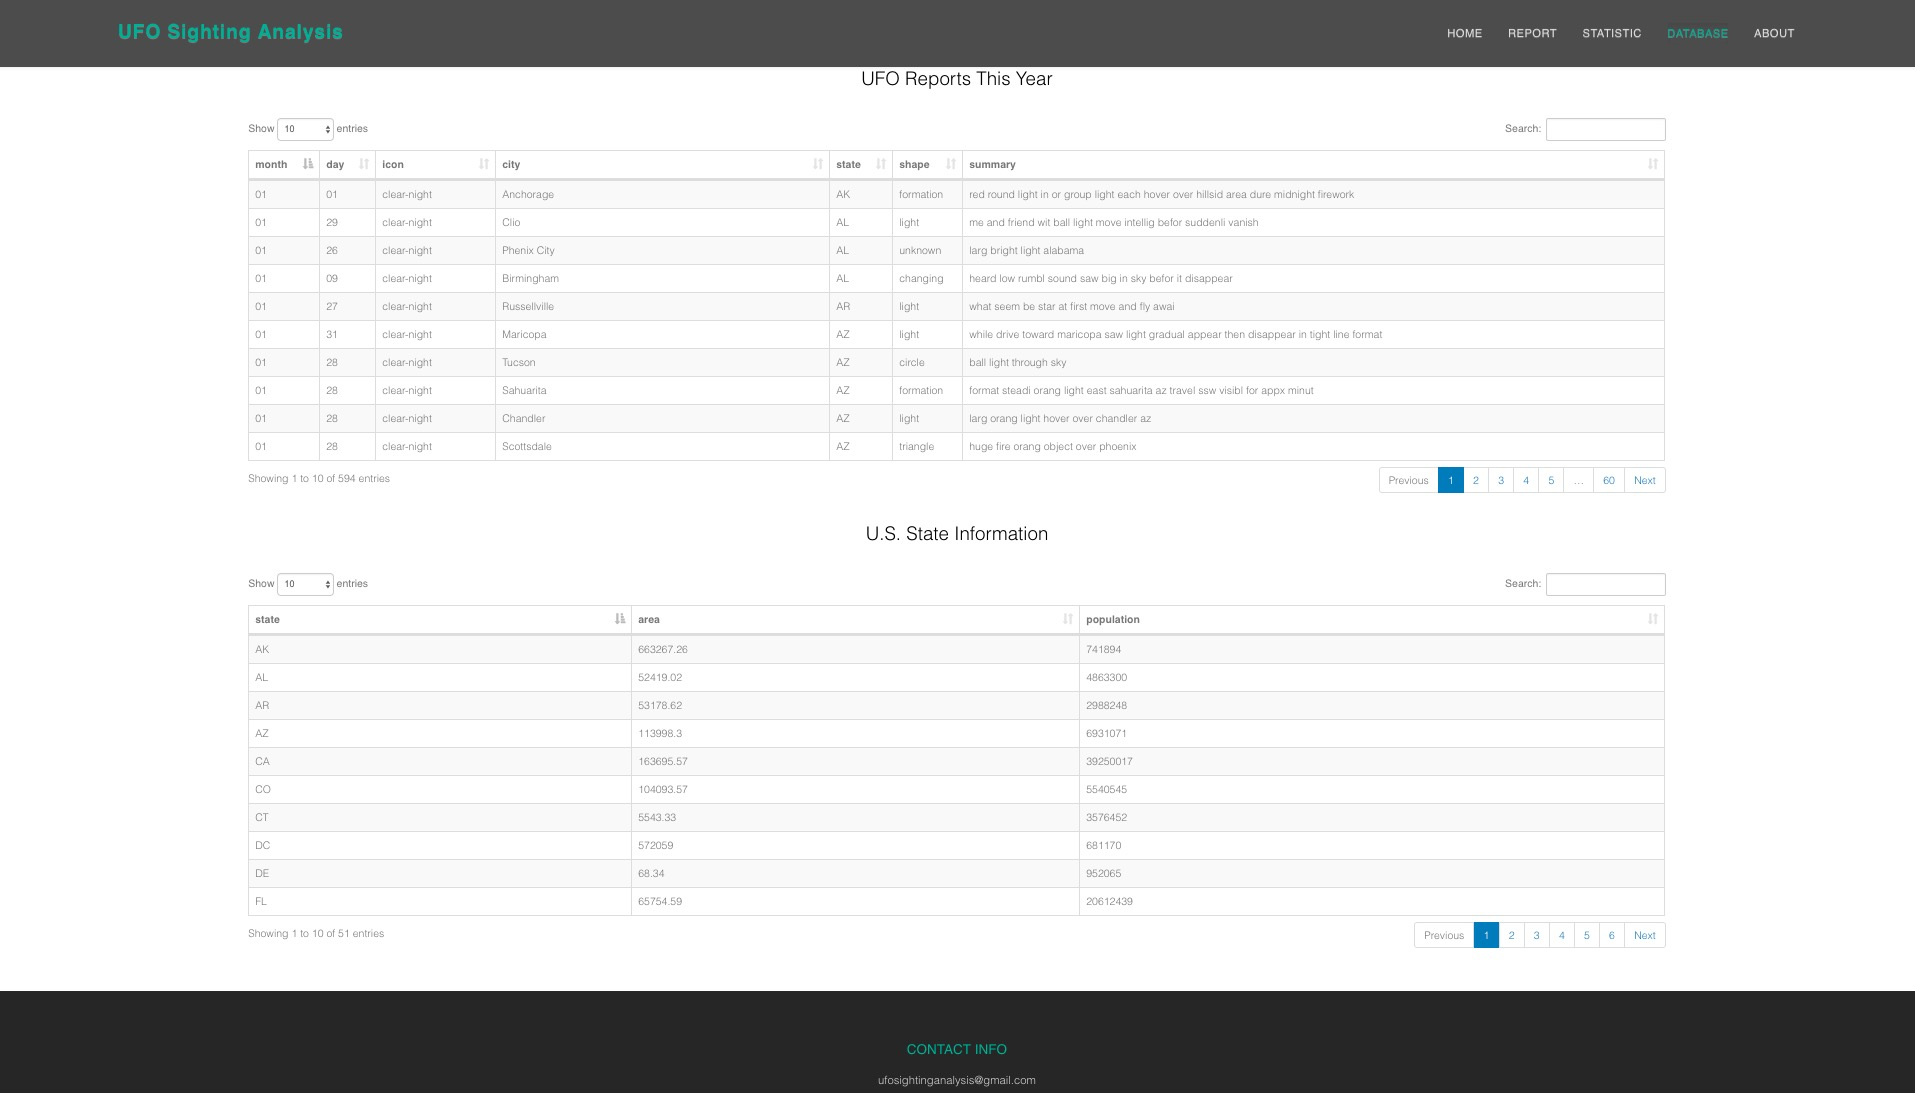
\includegraphics[width=1\textwidth]{figure/database.jpg}
\end{minipage}
}
\caption{home, statistic and database page}
\end{figure}

The home page of our website is shown in figure \ref{home}. There are three major functions of our website --- reporting UFO sighting, viewing statistic results, viewing database. Report page displayed in figure \ref{report} requires users to enter some information about their sightings: where, when, how long, what shape and their own summary. By clicking complete button, we will gather their reports' data and calculate their credibility by machine learning model illustrated in section \ref{ml}. Figure \ref{feedback} is a possible feedback to users. The classifier result is the possibility calculated by four classifiers separately. They vote in average to give out the final grade of user report. Numeric information lists other numeric features we gained from their report information. Information contribution is the proportion of grades between numeric and summary classifiers:
$$
sum\_log + sum\_tree : num\_svm + num\_tree
$$
Finally, we mark out user sighting against the accumulative UFO sighting distribution around U.S in a heat map. 



\begin{figure}[H]
\centering 
\subfigure[report page]{\label{report}
\begin{minipage}[b]{0.8\textwidth}
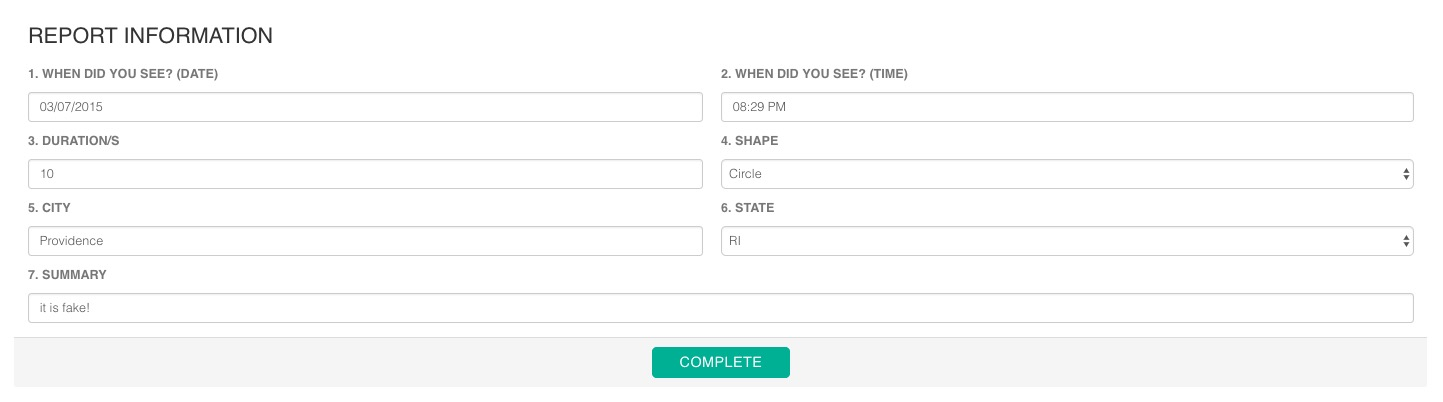
\includegraphics[width=1\textwidth]{figure/report.jpg}
\end{minipage}
}
\subfigure[feedback]{\label{feedback}
\begin{minipage}[b]{0.8\textwidth}
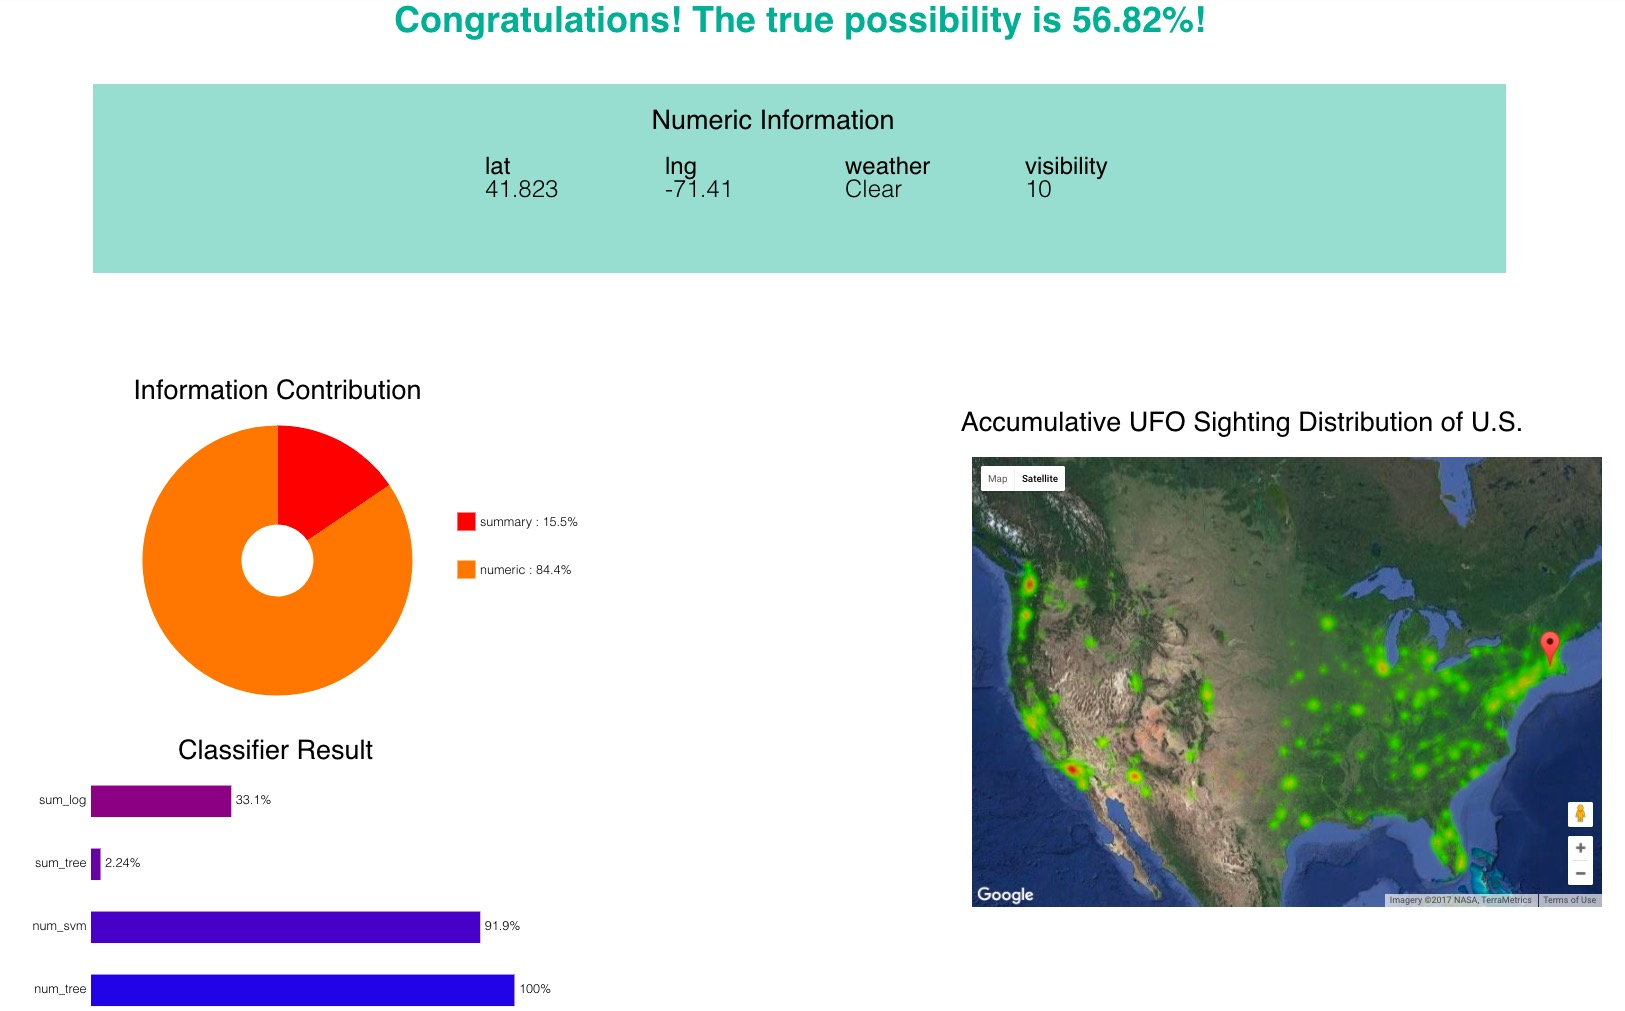
\includegraphics[width=1\textwidth]{figure/feedback.jpg}
\end{minipage}
}
\caption{report page}
\end{figure}

Statistic page in figure \ref{stats} shows our analysis results described in section \ref{statistic}. We use crossfilter~\cite{dcjs} to provide instant feedback to user interaction. Database view exhibits in figure \ref{database} uses DataTable~\cite{datatable} To show UFO reports in current year, as well as population and area information of U.S. that we used for machine learning.

\section{Challenges}\label{challenge}
To be honest, UFO data is really difficult to process and analyze. There are limited number of reports, and it's difficult to find out suitable models along with correct labels to predict. Actually we have tried many other ways, all of which finally failed to achieve satisfactory results.

\begin{figure}[H]
    \centering
    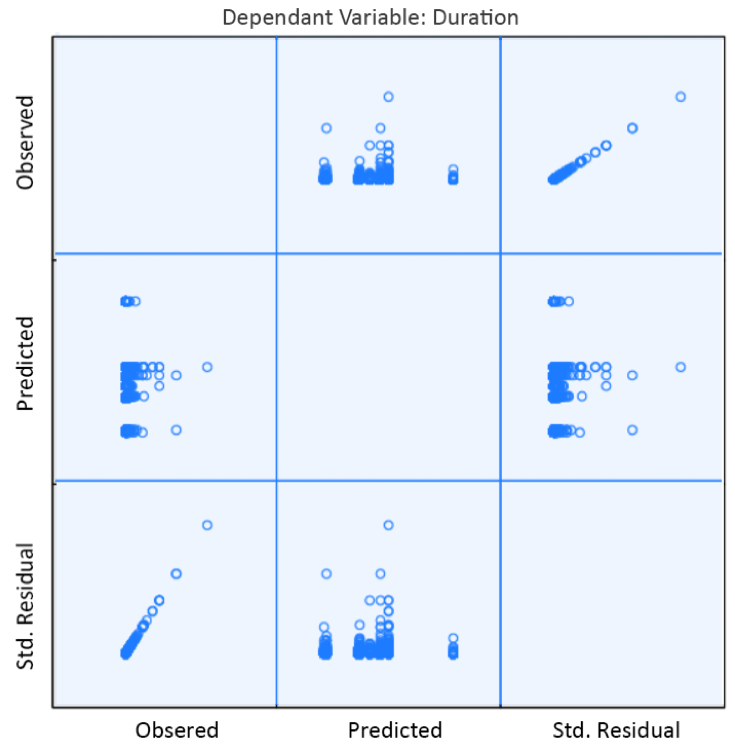
\includegraphics[width=7cm]{figure/correlation.png}
    \caption{intercept + weather}
    \label{correlation}
\end{figure}

At first, we try to predict duration, shape or location based on other features. However, when we do statistic analysis on a variety of meteorological features (temperature, wind speed, humidity, visibility, etc.,), geographical features along with the UFO reports data, most of them do not have significant correlations with other features of UFO reports data. For example, figure \ref{correlation} indicates the weak correlation between other features and duration of UFO appearances.

We have tried a lot of machine learning algorithms to detect fake reports. One approach is unsupervised learning --- clustering true and fake reports. However, as our training result shows, the internal cluster measures~\cite{clustermeasure} are not good, actually only 0.2 out of 1.~\footnote{$ 1 - \frac{compactness}{separation} $} Another way is to convert a classification problem on imbalanced data to an outlier detection problem only on positive data. We use one-class SVM to model true reports only. Based on true report boundary gained above, we use this model to detect which report is outlier,i.e., out of boundary. However, this method only generates a detecting accuracy slightly greater than 50\%, which is absolutely unacceptable.
\section{Conclusion \& Future Work}\label{conclusion}

According to our discussion in previous sections, we can draw following conclusions:

\begin{itemize}
    \item   Many UFO sightings occur at night, between 9 PM and 12 PM during a day, no matter whether it is clear or partly-cloudy. 
    \item   Sighting distribution across U.S. are imbalanced. States that near lakes, deserts and oceans tend to report more UFO sightings. California reports the most sightings, which also gets highest estimated marginal means of sighting duration.
    \item   Whether an UFO sighting report is true or just a hoax has close relationship to numeric features we extract. By using location information, time of a day, UFO shapes, weather conditions, our models can detect fake reports with a relatively high accuracy.
    \item   For text features, the word "reptile" has the biggest positive score, while the word "meteor" has the biggest negative score. 
    \item   Total UFO sighting number increases as year goes by, although slightly decreased recently. By using population and year as independent variable, our regression model predicts that there maybe 5589 UFO sightings in 2017.
\end{itemize}

Many further work can be done on UFO sighting data research. First and foremost is to find a better way to label data. NUFORC labeled data manually based on other information. For example, if a sighting's description and environment conditions are similar to satellite launching, they may label it as a fake report. It is possible to build a machine learning model based on related news analysis, which could label UFO reports automatically and more accurately.

Another thing is that we believe UFO sightings are related to many other different factors, like economy and vegetation. Consider what we derived in section \ref{statistic}. We conclude that California has more UFO sightings than the other states because of topographical features of desert and coast. But is this the truth? Is it possible this conclusion results from it's great economy, or any other conditions that is unique for the Golden State? We don't know. Many other data need to be collected, some of which even need some field research. 

After all, we believe UFOs, or aliens, do exist. But finding out rules of their occurrence on Earth is really difficult. Hope our work on analyzing sightings across U.S. could help further studies on this field.





\section{Acknowledgements}\label{ack}

We wish to show our profound gratitude to professors teach us data science. Most of our methods are learned from their great lectures. Meanwhile, we are grateful to our TAs', especially Michael Xu, our mentor TA, selfless help.
\begin{thebibliography}{9}
\bibitem{nuforc} 
\href{http://www.nuforc.org/}{The National UFO Reporting Center}

\bibitem{googlemap}
\href{https://developers.google.com/maps/documentation/javascript/}{Google Map API}

\bibitem{darksky}
\href{https://darksky.net/dev/docs}{Dark Sky API}

\bibitem{census}
\href{https://www.census.gov/}{United States Census Bureau}

\bibitem{dcjs}
\href{https://dc-js.github.io/dc.js/}{dc.js - Dimensional Charting Javascript Library}

\bibitem{datatable}
\href{https://datatables.net/}{DataTable}

\bibitem{clustermeasure}
Liu, Yanchi, et al. "Understanding of internal clustering validation measures." Data Mining (ICDM), 2010 IEEE 10th International Conference on. IEEE, 2010.
\end{thebibliography}
\end{document}